\chapter{\ac{lora} Ad-Hoc Simulator}
With an understanding of \ac{lora}'s performance - the next stage is to understand how \ac{lora} performs in an ad-hoc network. This section proposes a specialised Ad-Hoc \ac{lora} simulator, using models directly from \ac{phy} testing, as well as literature. It supports both scripted access for repeatable statistical testing and provides a GUI overlay for visually identifying system behaviour and performance. 

\textit{Full source code is available in the project design archive.}

\section{Model}
\subsection{Overview}
The model is considered as three main components, the environment, the radios, and time. The environment is responsible for understanding radio placement and the propagation channel between radios. Radios create new transmissions and poll the environment for existing transmissions, which they then attempt to receive. The simulator supports both the theoretical \ac{lora} radio (modelled from the datasheet), and the empirically defined RFM95W. Time progression of the system is modelled using the activity-oriented paradigm; this is where time is considered as small sequential slices at a selectable granularity (e.g. 1ms, 5ms, 10ms). For every simulation tick, the time-slice increments and any events that have occurred or are occurring within that time slice are handled. Unlike an event-driven approach, every time-slice is simulated, allowing for continuous receive behaviour close to that of a real-world scenario; the drawback being that it is processor intensive.


\subsection{Radio Model}
\subsubsection{Transmitting}
When a packet is transmitted, it is modelled in terms of start time, airtime and emanating location. Each time-slice the environment will poll each radio to collate all ongoing transmissions in the environment; this is the list which radios attempt to receive from and interference models are calculated for. If a radio's location changes between time-slices, the emanating location will be re-evaluated each time, however, the Doppler effect is not modelled because it has little effect for  on \ac{lora} at expected movement speeds \cite{3YP:DOPLER_EFFECT}. Transmission airtimes are calculated using the equations detailed in Section \ref{sec:airtime}.

\subsubsection{Receiving}
Every time-slice, a radio, provided it is not transmitting, will fill its receive buffer with a partial receive of the strongest receivable transmission (highest \ac{snr}) in the environment. For \ac{lora} transmissions, receivable implies the same \ac{sf}, \ac{bw} and \ac{cf} values are used. If multiple receivable signals are present, and the radio is not synchronised with a signal, the strongest will be captured. A small advantage is provided to favour receiving synchronised transmissions to support Class B and C collision scenarios. Class E collisions are handled by randomly adjusting receive \ac{snr}s slightly so that no preference is made between two signals with similar strength. Simulator collision results, as verified by the \texttt{TestCollision} class, are seen in Table  \ref{tab:sim_collisions}.

\begin{table}[H]
\centering\small
\caption[Simulator results for collision scenarios]{Results for collision scenarios defined in Table \ref{tab:collisions}, when modelled in the simulator. All scenarios are modelled correctly for all \ac{sf}s.}
\begin{tabular}{c|cc|c|c}
    \toprule
    \textbf{ID} & \textbf{Time} & \textbf{Power} & \textbf{Status} & \textbf{Metadata Status}\\
    \midrule\addlinespace
    A & $B_{start} > A_{\text{IP}}$ & $A_{\text{\ac{rps}}} \geq B_{\text{\ac{rps}}}$ & Receive A &  \cellcolor{green!25}\texttt{SUCCESS} \\
    B & $B_{start} > A_{\text{IP}}$ & $A_{\text{\ac{rps}}} < B_{\text{\ac{rps}}}$ & Receive A &  \cellcolor{green!25}\texttt{SUCCESS} \\
    C & $B_{start} > A_{\text{IP}}$ & $A_{\text{\ac{rps}}} \ll B_{\text{\ac{rps}}}$& CRC Fail A &  \cellcolor{green!25}\texttt{PAYLOAD\_COLLISION}  \\
    D & $B_{start}$ \textit{inside} $A_{\text{IP}}$ & $A_{\text{\ac{rps}}} \leq B_{\text{\ac{rps}}}$ & Collision &  \cellcolor{green!25}\texttt{PREAMBLE\_COLLISION} \\
    E & $B_{\text{IP}} \approx A_{\text{IP}}$ & $A_{\text{\ac{rps}}} \approx B_{\text{\ac{rps}}}$ & Collision &  \cellcolor{green!25}\texttt{PAYLOAD\_COLLISION}  \\
    F & $B_{\text{IP}} \approx A_{\text{IP}}$ & $A_{\text{\ac{rps}}} \gg B_{\text{\ac{rps}}}$ & Receive A &  \cellcolor{green!25}\texttt{SUCCESS} \\
    \addlinespace\bottomrule
\end{tabular}
\label{tab:sim_collisions}
\end{table}

Synchronisation is achieved when the important preamble of a signal (last 6.25 symbols) is in the receive buffer and demodulated successfully. Attempted demodulation occurs at the end of each time-slice and must pass at three stages to successfully receive a signal. If any stage fails the latter stages will not occur, but the signal will be unreceivable and may still interfere. The stages are:
\vspace{-2mm}
\begin{enumerate}[label=\textbf{S\arabic*}]
  	\item {When a transmission's first important preamble symbol is seen.	 \\Start of synchronisation.} \label{demod_s1}
  	\item {At the end of the transmission's preamble. At this point the radio is synchronised with a signal and is aware that it is receiving \cite{3YP:LORA_SX12}.} \label{demod_s2} 
  	\item {At the end of the transmission. Check for successful receive.} \label{demod_s3} 
\end{enumerate}
\vspace{-2mm}

\ref{demod_s1} purely checks if the signal is strong enough using the radio's demodulation curve. Failure will result in \texttt{NO\_PREAMBLE}, indicating a weak preamble. \ref{demod_s2} and \ref{demod_s3} also verify that enough of the transmission is present. This is required because it is possible that another powerful transmission has started filling the receive buffer - at this stage other signals are considered interference. For \ref{demod_s2}, 80\% of the signal must be preamble from the correct signal. For \ref{demod_s3} the amount of interference must not exceed the \ac{cr}'s capability (Table \ref{cr_effect}); this resembles burst-interference disrupting a portion of the signal. Failure due to interference will result in a \texttt{PREAMBLE\_COLLISION} or a \texttt{PAYLOAD\_COLLISION} for \ref{demod_s2} and \ref{demod_s3} respectively. Likewise a demodulation failure will result in either \texttt{NO\_PREAMBLE} or \texttt{WEAK\_PAYLOAD}. These statuses are simulation metadata, the radio does not necessarily know the failure details or that it even occurred - a mapping of metadata to radio knowledge is seen in Table \ref{tab:sim_metadata_translation}.

\begin{table}[H]
\centering\small
\caption[Simulator metadata to radio status mappings]{Mappings of simulator receive statuses to those the radio would see.}
\begin{tabular}{c|cc}
    \toprule
    \textbf{Metadata Status} & \textbf{Radio Status} & \textbf{Radio Aware} \\
    \midrule\addlinespace
	\texttt{NO\_PREAMBLE} & N/A & No \\
	\texttt{PREAMBLE\_COLLISION} & Collision & Yes \\
	\texttt{WEAK\_PAYLOAD} & \ac{crc} Fail & Yes \\
	\texttt{PAYLOAD\_COLLISION} & \ac{crc} Fail & Yes \\
	\texttt{SUCCESS} & Receive & Yes \\
    \addlinespace\bottomrule
\end{tabular}
\label{tab:sim_metadata_translation}
\end{table}

The mentioned demodulation curve varies depending on whether the theoretical model or the empirical RFM95W is used; only the latter is considered here. The transmission strength is calculated as the log-mean \ac{snr} of all its partial receives. The corresponding $p=\text{\ac{prp}}_{\text{\ac{snr}}}^{\text{\ac{sf}}}$ is found from the the best-fit sigmoid. If the \ac{snr} is close to $D_L$, $p$ is randomly adjusted to emulate high-variance behaviour. Demodulation success is then determined as a random chance with success $p$. The demodulation curves for receives at various \ac{snr}s are plotted in Figure \ref{fig:sf_sim_plot} (output generated by \texttt{FreeSpacePlot} class).

\begin{figure}[H]
    \centering
   	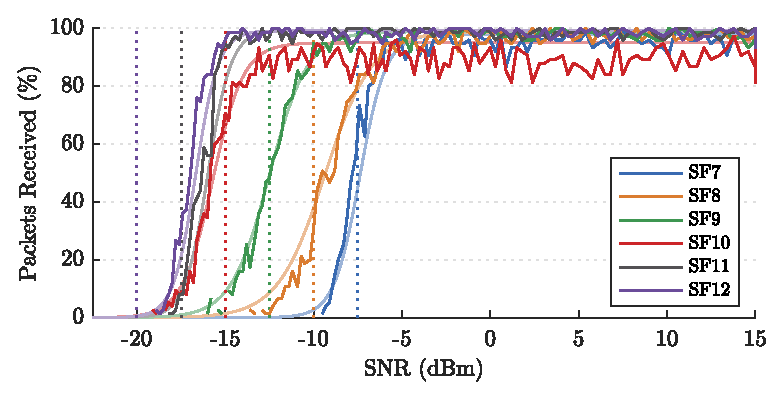
\includegraphics{Figures/sf_sim_plot}
    \caption[Simulator demodulation performance]{
    	Simulator demodulation performance, assessed as \ac{prp} for increasing \ac{snr}. Each point is the result of 75 transmitted packets at the respective \ac{snr}. The faded lines indicate the empirical fit curves from Section \ref{sec:demodulation_performance}. 
    }
    \label{fig:sf_sim_plot}
\end{figure}

\subsubsection{CAD}
\ac{lora}'s \ac{cad} process requires the ability to poll the receive buffer for a preamble symbol. When the process is invoked, the initial contents of the receive buffer are emptied as previous receive data cannot be used. A symbol's length of receive buffer is then captured (Equation \ref{eq:symbol_time}) and then the \ac{cad} search result is returned after the average processing time ($0.85\cdot S_T$) \cite{3YP:LORA_SX12}. Activity is detected if at least 80\% of the receives in the buffer are preamble symbols and a standard demodulation curve check passes. When the process is complete the full receive buffer is dumped as it cannot be used for receives.

\subsection{\ac{rps} ($R_P$) \& \ac{snr} Model}
The actual receivable signal power of a transmission is derived from the link budget equation, Equation \ref{eq:rp} explicitly repeats this for the factors modelled.
\begin{equation}
\label{eq:rp}
	R_P = TX_{power} + TX_{gain} + RX_{gain} - P_{loss}^{TX\rightarrow RX}
\end{equation}
Gains at the receiver and transmitter end are broken down into fixed antenna gains and cable losses. The path loss ($P_{loss}$) is broken down into free-space loss and object loss. A global free-space model is used for the environment, selectable at creation. Although adding any new model is straightforward,  built-in options include those defined in Section \ref{sec:environment_propagation}: E-FSPL, FSPL, PE. 

\begin{figure}[H]
    \centering
   	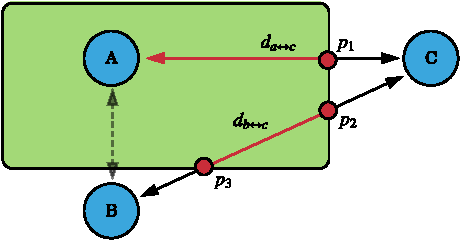
\includegraphics{Figures/obstacle_diagram}
    \caption[Object path loss scenarios]{
    	Scenarios for LOS path loss whilst passing through objects.   
    }
    \label{fig:object_path_loss}
\end{figure}

Objects are entities in the environment, which will possess their own propagation model; built-in models include: COST235, Weissberger and the ITU-R. Forests are a type of built-in object; these can take any 2D shape and use the ITU-R model with a $\beta$ multiplier. All this combined allows the path loss curves from Section \ref{sec:environment_propagation} to be recreated. Of course in a real environment, it is likely that not all radio transmissions will pass through the same obstacles. There is no perfect way to handle this, the closest would be the one woodland terminal model \cite{3YP:RF_BOOK} but this sets severe limits; one radio must be in the object and the other outside with no other obstacles in the path. Therefore a more approximate approach is taken. In short the total $P_{loss}$ is sum of the free-space loss and the segment of the propagation curve from the obstacle.  Using Figure \ref{fig:object_path_loss} as a scenario reference, the following are examples of extra $P_{loss}$ due to obstacles. Equation \ref{eq:path_loss_a_c} calculates for $A\leftrightarrow C$ where one radio is in the obstacle.
    	\begin{equation}
    	\label{eq:path_loss_a_c}
    	\begin{split}
    	    	P_{loss \text{ (Object)}}^{A\rightarrow C} = P_{loss}^{A\rightarrow p_1}
    	\end{split}
    	\quad\leftrightarrow\quad
    	\begin{split}
    		    P_{loss \text{ (Object)}}^{C\rightarrow A} = P_{loss}^{C\rightarrow A}-P_{loss}^{C\rightarrow p_1}
    	\end{split}
    	\end{equation}
    	Equation \ref{eq:path_loss_b_c} calculates for $B\leftrightarrow C$ where the transmission completely passes through the object.
    	\begin{equation}
    	\label{eq:path_loss_b_c}
    	\begin{split}
    	        P_{loss \text{ (Object)}}^{B\rightarrow C} = P_{loss}^{B\rightarrow p_2}-P_{loss}^{B\rightarrow p_3}	
    	\end{split}
    	\quad\leftrightarrow\quad
    	\begin{split}
    	    	P_{loss \text{ (Object)}}^{C\rightarrow B} = P_{loss}^{C\rightarrow p_3}-P_{loss}^{C\rightarrow p_2}
    	\end{split}
    	\end{equation}
    
    As the method has large swings in path loss depending on whether obstacles are close to the receiver or transmitter, $\text{max}(P_{loss}^{TX\rightarrow RX}, P_{loss}^{RX\rightarrow TX})$ is taken; this means path loss will be the same regardless of the transmission direction -- interference differences may still mean that \ac{snr} varies. The model scales to any number of objects in the path. Note that fast-fading is abstracted into the demodulation curve of the receiver and is not modelled separately.  	

The channel power as seen by a receiver (\ac{rssi}) at a location, is modelled as the sum of: all `interfering' signal powers, the thermal noise floor ($T_N$), and the receiver noise figure ($N_f$). When attempting to receive a signal, its observed $R_P$ can removed from the \ac{rssi} calculation to provide the channel noise ($N$). The \ac{snr} can then be calculated as $R_P - N$. Interfering sources, narrowband or otherwise, are considered as those where the bandwidth used overlaps with the receive channel. As per \ac{lora}'s orthogonality defined in Section \ref{sec:sf_orthogonality}, a \ac{lora} transmission is only considered to interfere if the chirp rate is the same as that of the receive configuration.


\subsection{Protocol Testing Infrastructure}
Protocols are implemented the layer above the low-level radio behaviour using a listener infrastructure. When the time-slice increments, first the raw radio behaviour will occur, and then a `tick' process will be called on any listeners. These listeners can maintain their own state between ticks allowing them to schedule transmissions and handle received packets, ultimately allowing emulation of a full protocol stack. More implementation specific behaviour like radio movement can be emulated here or on a higher level listener. This is how all the protocols defined in Section \ref{sec:protocols} are implemented. The base listener class, \texttt{ProtocolTickListener}, provides methods for directly handling events that have occurred the previous tick (synchronisations, receives, CAD results), tracks received data, and handles protocol performance tracking (for testing). Statistics can be dumped with a by-radio perspective -- the number of  packets received by each radio and the reason for any failures. Or with a by-transmission perspective -- the number of receivers of each transmission and the reason for any failures. Outputs can be filtered to disregard failures of transmissions that are not `wanted' by a receiver (see Section \ref{sec:mac_considerations}).

The execution of an environment (and the radios within it) is handled by an \texttt{EnvironmentRunner}; this can step time by the configured granularity a number of times or run continuously. Execution occurs on a separate thread and employs listeners to allow external interaction either through a test harness or GUI. Events can be created and scheduled for execution at fixed times to allow for scripted test behaviour; there is built-in support for moving radios, sending transmissions and verifying the expected radio state; although, with full control over the system, any custom behaviour can be implemented. 


\section{Interface (GUI)}
The Java Swing interface acts largely as a wrapper for managing an \texttt{Environment} \texttt{Runner} and displaying the environment being executed. The full interface can be seen in Figure \ref{fig:sim_interface_main} with further examples in Appendix \ref{sec:simulator_pictures}. User controls are provided for managing environment time, choosing presets and protocols, and accessing statistics. The graphical view, which has full support for panning and zooming, displays the environment's: objects, radios and transmissions. Objects are drawn using their obstruction shape (and specified attributes). Radios are blue circles when transmitting and grey otherwise. Transmission routes are displayed for the last received data in a radio's buffer as a line from transmitter to receiver with \ac{snr} indicated; preamble is identfied by a dotted line, payload as a solid line. The line will be grey if the receiver failed to synchronise with the preamble or red if the transmission was not the one the receiver is synchronised with. Otherwise, blue is used to indicate a data packet and orange as protocol overhead. Together visual cues provides an exact understanding of behaviour.

\begin{figure}[H]
    \centering
   	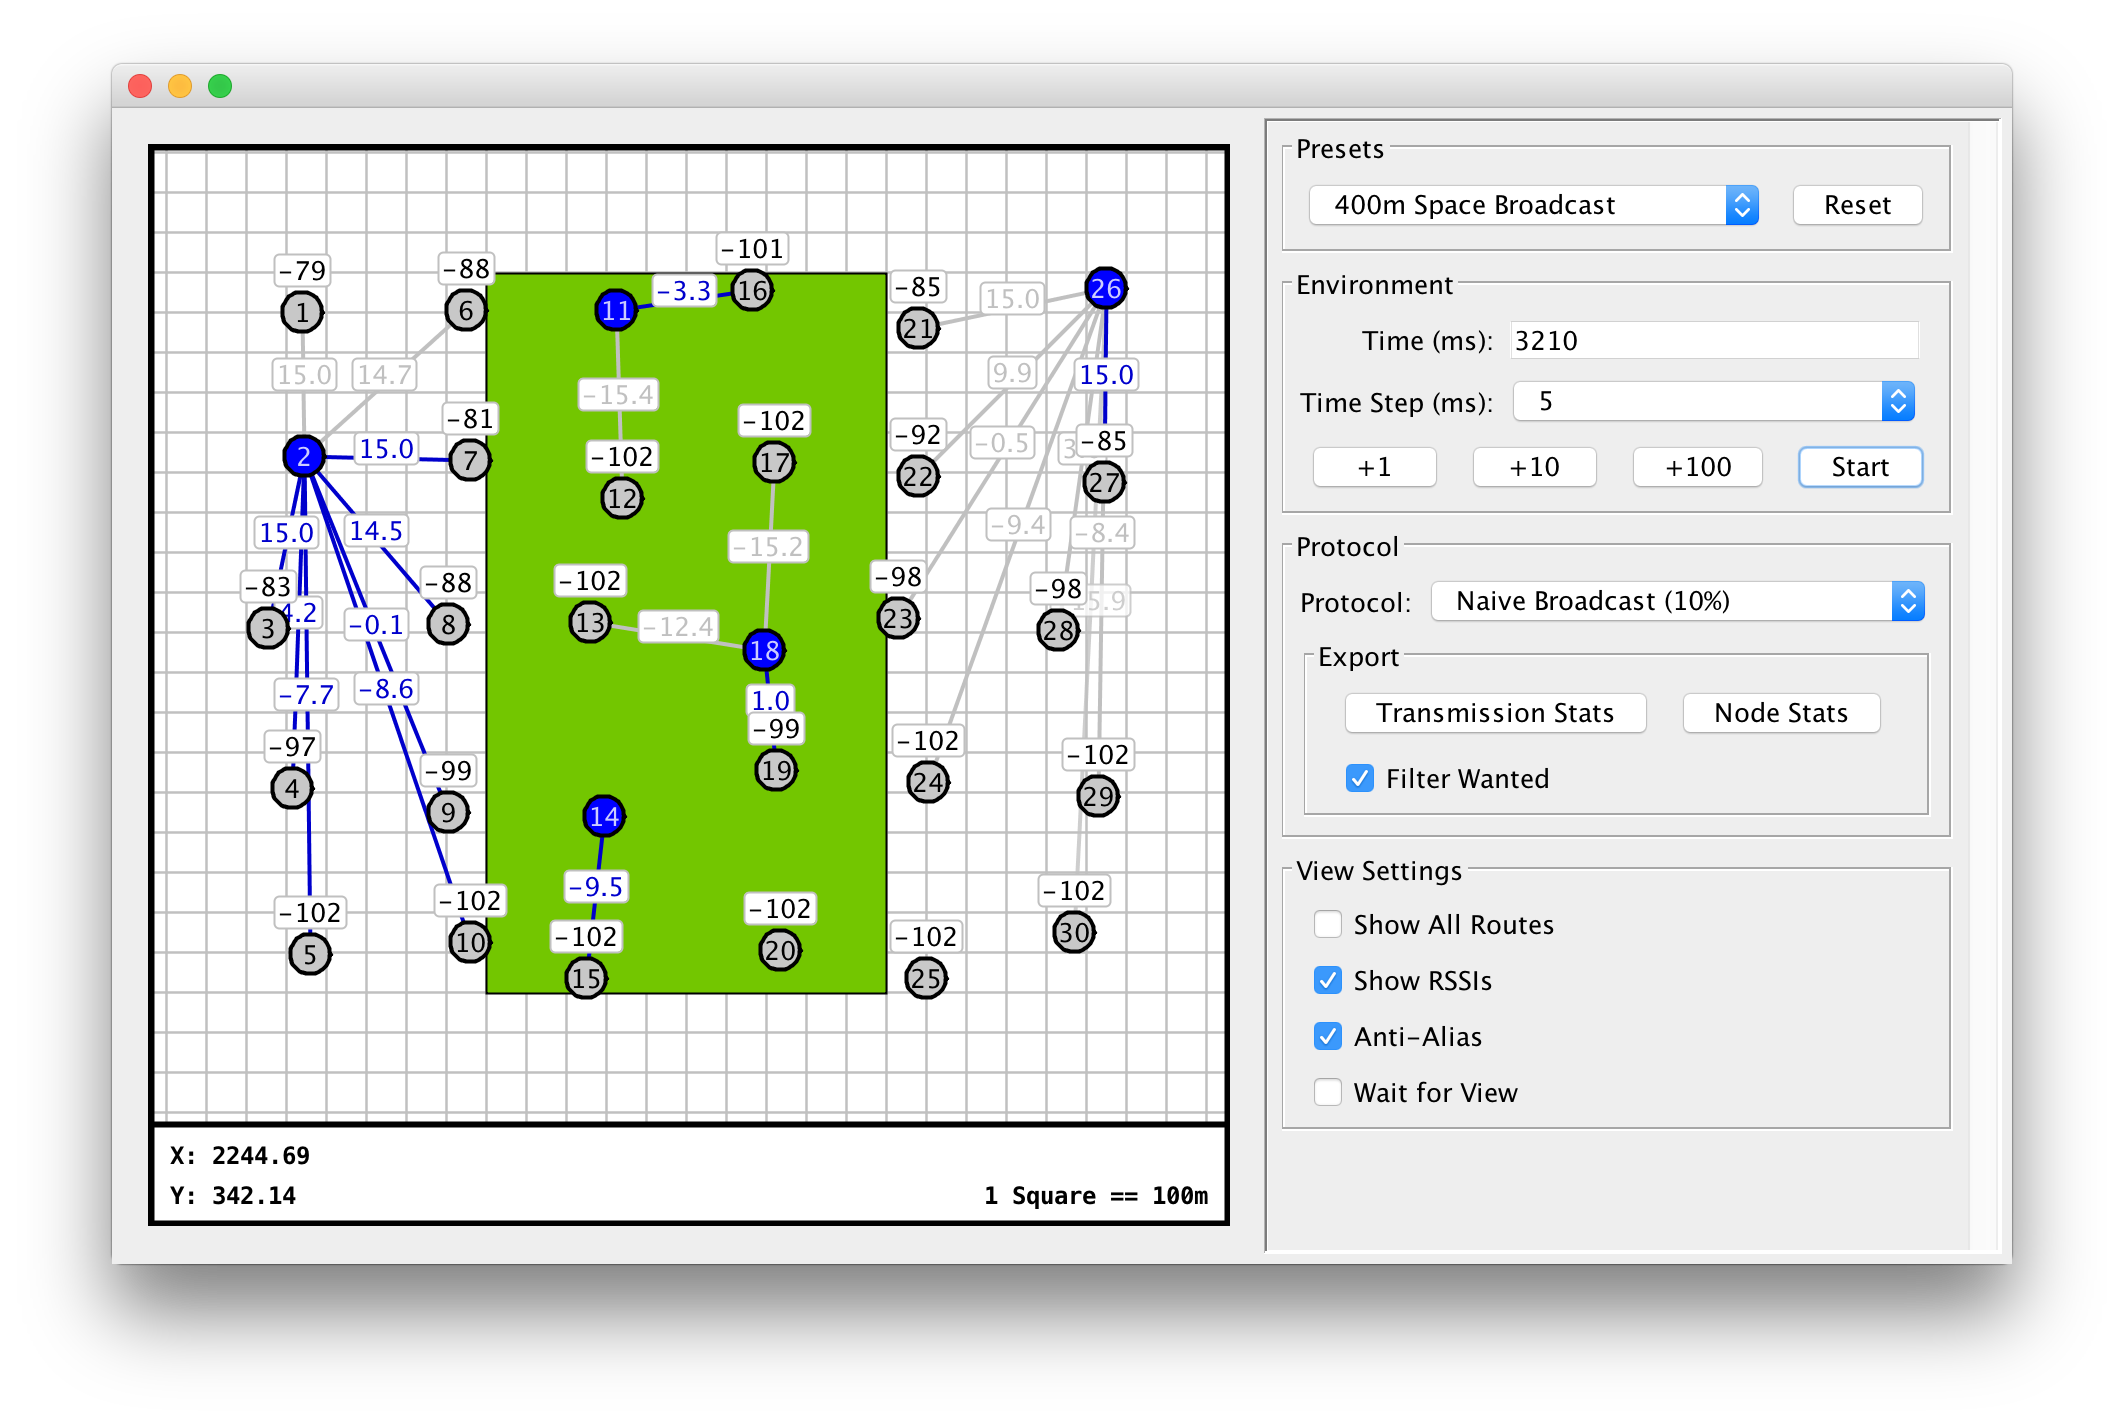
\includegraphics[width=\textwidth]{Figures/simulator_main}
    \caption[Simulator GUI example]{ 
    	Simulator's GUI interface running the naive (ALOHA) protocol.
    	}
    \label{fig:sim_interface_main}
\end{figure}





%Network simulations allow early assessment of basic protocol performance in controlled environments. Off-the-shelve simulation tools, such as ns-3\footnote{ns-3, https://www.nsnam.org}, offer very broad feature sets but consequently, creating an implementation with novel features, such as those present with \ac{lora} (\ac{cad}, orthogonal \ac{sf}s), is not trivial. Therefore, it was deemed more time-effective to create a specialised ad-hoc \ac{lora} simulator, using models from the \ac{phy} testing, with a subset of features relevant to the testing scenarios. The created simulator is detailed in the next section. The non-interface mode was used for gathering statistical results. Whereas, the GUI overlay was used for visually identifying node behaviour to aid understanding of statistical test results.